\documentclass[fontsize=10pt,a4paper]{scrartcl}

\usepackage{../../styles/myusepackages}
\usepackage{../../styles/mypythonstyle}
\usepackage{../../styles/myMCquestions}
\usepackage{../../styles/myframedenv}
%If graphics is listed before,some problems arise
\usepackage{graphicx}

\usepackage[english]{babel}
\usepackage[english,verbose]{layout}
\hypersetup{pdflang={es-ES}}

\newcommand{\academicyear}{2023-2024}
%%%%%%%%%%%%%%%%%%%%%%%%%%%%%%%%%%%%%%%%%%%%%%%%
%%%%%%%%%%%% TITLE
\title{Programing in Python\\ TEMA 5}
\usepackage{etoolbox}
\makeatletter
\providecommand{\subtitle}[1]{% add subtitle to \maketitle
  \apptocmd{\@title}{\par {\Huge #1 \par}}{}{}
}
\makeatother
\subtitle{\Large{Funciones y testing}}
\author{Universidad Politécnica de Valencia}
\date{\academicyear{}}
%%%%%%%%%%%%%%%%%%%END TITLE%%%%%%%%%%%%%%%%%%%%%

\begin{document}
\maketitle
\tableofcontents


\chapter*{Prólogo}
\addcontentsline{toc}{chapter}{Prólogo}


¡Bienvenido a este libro de Python que te acompañará en el tema de programación durante el primer semestre de tus estudios universitarios!

Este libro se inspira en dos obras de código abierto:\textit{Python for Everybody} de Charles Severance \cite{severance2016python} y \textit{Think Python: How to Think Like a Computer Scientist} de Allen Downey \cite{downey2016thinkpython}. Estos libros han compartido su conocimiento bajo licencias de Creative Commons, formando la base del contenido de este libro.

La motivación para crear este libro surge de la necesidad de comprender sólidamente las pruebas (o el «testing») en la educación de programación. Creemos que las pruebas son una habilidad esencial en el mundo de la programación, pero sorprendentemente, este aspecto crucial a menudo se pasa por alto en los libros de programación para principiantes. Con el libro que tienes en tus manos, buscamos cambiar eso.

Integrar el «testing» en un curso de programación para principiantes no es fácil. Es por eso que utilizamos el innovador enfoque TILE \cite{10132188} «Test Informed Learning with Examples» o el Aprendizaje Informado por Pruebas con Ejemplos. El enfoque TILE se centra en integrar las pruebas de software en tu experiencia de programación introductoria de manera efectiva y placentera. TILE fue desarrollado con el generoso apoyo y financiamiento del proyecto Erasmus+ QPeD (número de contrato 2020-1-NL01-KA203-064626) y del proyecto ENACTEST (número de proyecto 101055874).

Con TILE, las pruebas se convierten en una parte integral de tu trayecto de programación desde el principio. Creemos firmemente que las pruebas no deben ser una idea secundaria, sino un aspecto esencial de tu proceso de codificación. Por eso te presentamos las pruebas desde el primer programa de ejemplo que encuentres.

Nuestro objetivo es dotarte del conocimiento y las habilidades para que te conviertas en un programador Python competente, armado con el poder de las pruebas para crear programas de alta calidad.

Así que, mientras te sumerges en el emocionante mundo de Python, recuerda que este libro está aquí para guiarte paso a paso en el dominio tanto de la programación como de las pruebas. Juntos, embarquémonos en este viaje mientras exploramos las maravillas de Python y el arte de las pruebas de software.

¡Feliz aprendizaje!

Tanja Vos
(tvos@dsic.upv.es)

\hypertarget{functionchap}{%
\section{Function calls}\label{functionchap}}

\index{función, llamada a}

In the programming context, a \emph{function} is a sequence of statements that perform an operation and are given a name. When a function is defined, the name and the sequence of statements are specified. Later, you can ``call'' the function by that name. We have already seen an example of a \emph{function call}:

\begin{Verbatim}[frame=single]
>>> type(32)
<class 'int'>
\end{Verbatim}


The function name is \pythoninline{type}. The expression in parentheses is called the \emph{argument} of the function. The argument is a value or variable that is passed to the function as an input parameter. The result of the \pythoninline{type} function is the type of the argument.

\index{paréntesis!argumento in}

It is common to say that a function ``takes'' (or receives) an argument and ``returns'' a result. The result is called \emph{value return}.

\index{argumento} \index{valor de retorno}

\section{Built-in functions)}\label{funciones-predefinidad}

Python provides a large number of built-in functions, which can be used without having to write them first. The creators of Python have written a set of functions to solve common problems and included them in Python for us to use.

The functions \pythoninline{max} and \pythoninline{min} will give us the largest and smallest value of a list, respectively:

\begin{Verbatim}[frame=single]
>>> max('Hello world!')
  'w'
>>> min('Hello world!')
  ' '
\end{Verbatim}

The \pythoninline{max} function tells us what the ``largest character'' in the string is (which is the letter ``w''), while the \pythoninline{min} function returns the smallest character (which in that case is a space). Remember that the string comparison uses the ASCII codes of the characters. These codes can be found using the predefined function \pythoninline{ord}:

\begin{Verbatim}[frame=single]
>>> ord(" ")
  32
>>> ord("a")
  97
>>> ord("u")
  117
>>> ord("H")
  72
>>> ord("!")
  33
\end{Verbatim}

Another very common built-in function is \pythoninline{len}, which tells us how many elements are in its argument. If the argument of \pythoninline{len} is a string, it returns the number of characters in the string.

\begin{Verbatim}[frame=single]
>>> len('Hello world!')
  12
>>>
\end{Verbatim}

These functions are not limited to strings. They can operate on any set of values, as we will see in the following chapters.

\begin{Verbatim}[frame=single]
>>> len([1,2,3,4,5]) #a list
  5
>>> len({1:"one", 2:"two", 3:"three"})  #a dictionary
  3
\end{Verbatim}

Predefined function names should be treated as if they were reserved words (i.e. avoid using \pythoninline{max} as a variable name).

\hypertarget{funciones-de-conversiuxf3n-de-tipos}{%
\section{Type conversion functions}\label{funciones-de-conversiuxf3n-de-tipos}}

\index{conversión!tipo} \index{tipo, conversión de}

Python also provides built-in functions that convert values from one type to another. The \pythoninline{int} function takes any value and converts it to an integer if it can, or complains if it can't:

\index{int, función} \index{función!int}

\begin{Verbatim}[frame=single]
>>> int('32')
  32
>>> int('Hello')
  ValueError: invalid literal for int() with base 10: 'Hello'
\end{Verbatim}

\pythoninline{int} can convert floating point values to integers, but does not round them; just cut and discard the decimal part:

\begin{Verbatim}[frame=single]
>>> int(3.99999)
  3
>>> int(-2.3)
  -2
\end{Verbatim}

\pythoninline{float} converts integers and strings to floating point numbers:

\index{float, función} \index{función!float}

\begin{Verbatim}[frame=single]
>>> float(32)
  32.0
>>> float('3.14159')
  3.14159
\end{Verbatim}

Finally, \pythoninline{str} converts its argument to a string:

\index{str, función} \index{función!str}

\begin{Verbatim}[frame=single]
>>> str(32)
  '32'
>>> str(3.14159)
'. 3.14159'
\end{Verbatim}

\hypertarget{funciones-matemuxe1ticas}{%
\section{Math functions (the math module))}\label{funciones-matemuxe1ticas}}

\index{math, función} \index{función!math} \index{módulo}
\index{módulo, objeto}

Python has a math module \texttt{(math)}, which provides most of the usual math functions. Before we can use the module, we need to import it:

\begin{Verbatim}[frame=single]
>>> import math
\end{Verbatim}

This statement creates a \emph{module object} called math. If you print the module object, you get some information about it:

\begin{Verbatim}[frame=single]
>>> print(math)
  <module 'math' (built-in)>
\end{Verbatim}

The module object contains the functions and variables defined in the module. To access one of those functions, you need to specify the module name and the function name, separated by a period. This format is called \emph{dot notation}.

\index{notación punto}

\begin{python}[frame=single]
import math

relation = 25
decibels = 10 * math.log10(relation)

radians = 0.7
height = math.sin(radians)
\end{python}

The first example computes the base 10 logarithm of a variable \pythoninline{relation}. The math module also provides a function called \pythoninline{log} that computes logarithms to the base \texttt{e}.

\index{log, función} \index{función!log} \index{sine, función}
\index{radián} \index{trigonométrica, función}
\index{función, trigonométrica}

The second example calculates the sine of the variable \pythoninline{radians}. The variable name is a hint that \pythoninline{sin} and the other trigonometric functions (\pythoninline{cos}, \pythoninline{tan}, etc.) take arguments in radians. To convert from degrees to radians, divide by 360 and multiply by \(2\pi\):


\pythonexternal{code/grados_a_radianes.py}


\begin{Verbatim}[frame=single]
>>> %Run 
  How many degrees do you want to convert to radians? 45
  45.0 degrees is 0.7071067811865475 radians
\end{Verbatim}

The expression \pythoninline{math.pi} takes the variable \pythoninline{pi} from the math module. The value of that variable is an approximation of \(\pi\), accurate to about 15 digits.

\index{pi}

\hypertarget{nuxfameros-aleatorios}{%
\section{Random numbers (the random module)}\label{nuxfameros-aleatorios}}

\index{aleatorio, número} \index{número, aleatorio}
\index{determinístico} \index{pseudoaleatorio}

From the same inputs, most programs will generate the same outputs every time, which is what we call \emph{deterministic} behavior. Determinism is usually a good thing, since we expect the same operation to always give us the same result. For certain applications, however, we will want the result to be unpredictable. Games are the obvious example, but there is more.

Making a program truly non-deterministic is not that easy, but there are ways to make it at least appear so. One of them is to use \emph{algorithms} that generate \emph{pseudo-random} numbers. Pseudo-random numbers are not truly random, since they are generated by a deterministic operation, but if we only look at the numbers it is almost impossible to distinguish them from truly random ones.

\index{random, módulo} \index{módulo!random}

The \texttt{random} module provides functions that generate pseudo-random numbers (which we will simply call ``random'' from now on).

\index{random, función} \index{función!random}

The \pythoninline{random} function returns a random float number between 0.0 and 1.0 (including 0.0, but not 1.0). Each time \pythoninline{random} is called, the next number in a long series is returned. To see an example, run this loop:

\begin{python}[frame=single]
import random

for i in range(10):
    x = random.random()
    print(x)
\end{python}

This program produces the following list of 10 random numbers between 0.0 and (but not including) 1.0.

\begin{Verbatim}[frame=single]
0.11132867921152356
0.5950949227890241
0.04820265884996877
0.841003109276478
0.997914947094958
0.04842330803368111
0.7416295948208405
0.510535245390327
0.27447040171978143
0.028511805472785867
\end{Verbatim}

As an exercise, test this program on your system and see what numbers you get.

The \pythoninline{random} function is just one of many that work with random numbers. The \pythoninline{randint} function takes the parameters \texttt{lower} and \texttt{upper}, and returns an integer between \texttt{lower} and \texttt{upper} (including both ends).

\index{randint, función} \index{función!randint}

\begin{Verbatim}[frame=single]
>>> random.randint(5, 10)
  5
>>> random.randint(5, 10)
  9
\end{Verbatim}

To choose an element from a sequence randomly, \pythoninline{choice} can be used:

\index{choice, función} \index{función!choice}

\begin{Verbatim}[frame=single]
>>> random.choice([1, 2, 3])
  2
>>> random.choice("hello world")
  'l'
\end{Verbatim}

The \texttt{random} module also provides functions to generate random values from various continuous distributions, including Gaussian, exponential, gamma, and a few more.

\hypertarget{auxf1adiendo-funciones-nuevas}{%
\section{Adding new features}\label{auxf1adiendo-funciones-nuevas}}

So far, we have only been using the built-in functions of Python, but it is possible to add new functions as well. A \emph{function definition} specifies the name of a new function and the sequence of statements that are executed when that function is called. Once a function is defined, it can be reused over and over again throughout the program.

\index{función} \index{función, definición} \index{definición!función}

Here's an example:

\begin{python}[frame=single]
def sample_chorus():
    print("I said maybe")
    print("You're gonna be the one that saves me")
    print("And after all")
    print("You're my wonderwall")
\end{python}

\pythoninline{def} is a keyword indicating that this is a function definition. The name of the function is \pythoninline{sample\_chorus}. The rules for function names are the same as for variables: letters, numbers, and some punctuation marks can be used, but the first character cannot be a number. You can't use a keyword as a function name, and you should also avoid having a variable and a function
with the same name.

\index{def, palabra clave} \index{palabra clave!def} \index{argumento}

Empty parentheses after the name indicate that this function takes no arguments. Later we will build functions that receive input parameters.

\index{paréntesis!vacíos} \index{cabecera} \index{cuerpo}
\index{indentado} \index{dos-puntos}

The first line of the function definition is called the \emph{header}; the rest is called the \emph{body}. The header must end with a colon (:), and the body must be indented. By convention, the indent is always four spaces. The body can contain any number of statements. The different parts of the functions can be seen in Figure \ref{fig:partes_funciones}.

\begin{figure}[t]
    \centering
    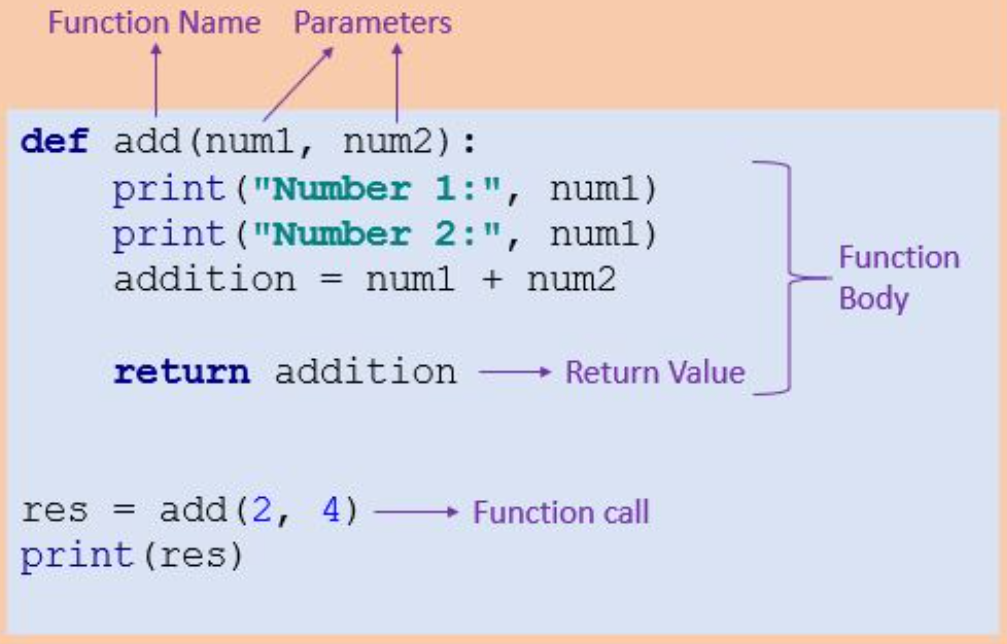
\includegraphics[width=\0.75\textwidth]{images/funciones_partes-eng.png}
    \caption{Functions in python}
    \label{fig:partes_funciones}
\end{figure}


\index{puntos suspensivos}
If you write a function definition in interactive mode in the console, the interpreter will display ellipses (\emph{\ldots{}}) to inform you that the definition is not complete:

\begin{Verbatim}[frame=single]
>>> def sample_chorus():
...     print("I said maybe")
...     print("You're gonna be the one that saves me")
...     print("And after all")
...     print("You're my wonderwall")
\end{Verbatim}

To end the function, you must enter an empty line (this is not necessary in a script).

When defining a function, a variable with the same name is created.

\begin{Verbatim}[frame=single]
>>> print(sample_chorus)
  <function sample_chorus at 0xb7e99e9c>
>>> print(type(sample_chorus))
  <type 'function'>
\end{Verbatim}

The value of \pythoninline{sample\_chorus} is \emph{function object}, which has type ``function''.

\index{función, objeto} \index{objeto!función}

The syntax for calling our new function is the same as we use for predefined functions:

\begin{Verbatim}[frame=single]
>>> sample_chorus()
  I said maybe
  You're gonna be the one that saves me
  And after all
  I said, I bet that you look good on the dance floor
\end{Verbatim}

Once a function has been defined, it can be used inside another. For example, to repeat the previous chorus, we could write a function called \pythoninline{repeat\_chorus}:

\begin{python}[frame=single]
def repeat_chorus():
    sample_chorus()
    sample_chorus()
\end{python}

And then call \pythoninline{repeat\_chorus}:

\begin{Verbatim}[frame=single]
>>> repeat_chorus()
  I said maybe
  You're gonna be the one that saves me
  And after all
  You're my wonderwall
  I said maybe
  You're gonna be the one that saves me
  And after all
  You're my wonderwall
\end{Verbatim}


\hypertarget{definiciuxf3n-y-usos}{%
\section{Definition and uses}\label{definiciuxf3n-y-usos}}

\index{función, definición}

Putting the code snippets from the previous sections together, the complete program would look something like this:

\begin{python}[frame=single]
def sample_chorus():
    print("I said maybe")
    print("You're gonna be the one that saves me")
    print("And after all")
    print("You're my wonderwall")

def repeat_chorus():
    sample_chorus()
    sample_chorus()

repeat_chorus()
\end{python}

This program contains two function definitions: \pythoninline{sample\_chorus} and \pythoninline{repeat\_chorus}. Function definitions are executed just like any other statement, but their result is to create objects of type function. Statements within each function are executed only when that function is called, and a function definition does not generate any output.

\index{use before def}

As you can imagine, it is necessary to create a function before it can be executed. In other words, the function definition must be executed before the function is called for the first time.

Shift the last line of the above program up, so that the function call appears before the definitions. Run the program and see what error message you get.

Move the function call back to the end, and put the \pythoninline{sample\_chorus} definition after the \pythoninline{repeat\_chorus} definition. What happens when you try that program?

\hypertarget{flujo-de-ejecuciuxf3n}{%
\section{Execution flow}\label{flujo-de-ejecuciuxf3n}}

\index{flujo de ejecución}

To make sure that a function is defined before using it for the first time, it is necessary to know the order in which the statements are executed, which is what we call the \emph{execution flow}.

Execution always starts at the first statement in the program. The statements are executed one by one, in order from top to bottom.

Function \emph{definitions} do not alter the flow of program execution, but remember that statements within a function are not executed until that function is called.

A function call is like a detour in the flow of execution. Instead of going to the next statement, the stream jumps to the body of the function, executes all the statements there, and then returns to where it left off.

This all sounds pretty straightforward, until you remember that one function can call another. When in the middle of a function, the program may have to execute the statements of another function. But when you're executing that new function, there may be even more functions to execute!

Fortunately, Python is able to keep track of where it is at any given moment, so that each time it completes a function's execution, the program returns to where it left off in the function that called it. When this takes you to the end of the program, it just ends.

What is the moral of this strange story? When you read a program, you don't always want to do it from top to bottom. Sometimes it makes more sense to go with the flow of execution.

\hypertarget{paruxe1metros-y-argumentos}{%
\section{Parameters and arguments}\label{paruxe1metros-y-argumentos}}

\index{parámetro} \index{parámetro!de función} \index{argumento}
\index{argumento de función}

Some of the built-in functions we've seen need arguments. For example, when \pythoninline{math.sin} is called, it is passed a number as an argument. Some functions need more than one argument: \pythoninline{math.pow} takes two, the base and the exponent.

Inside functions, the arguments are assigned to variables called \emph{parameters}. Here's an example of a user-defined function that takes one argument:

\index{paréntesis!parámetros entre}

\begin{python}[frame=single]
def show_twice(bruce):
    print(bruce)
    print(bruce)
\end{python}

This function assigns the argument to a parameter named \pythoninline{bruce}. When the function is called, it prints the value of the parameter (whatever it is) twice.

This function works with any value that can be displayed on the screen.

\begin{Verbatim}[frame=single]
>>> show_twice('Spam')
  Spam
  Spam
>>> show_twice(18)
  18
  18
>>> show_twice(math.pi)
  3.14159265359
  3.14159265359
\end{Verbatim}

The same composition rules that apply to built-in functions also apply to user-defined functions, so we can use any type of expression as an argument to \pythoninline{display\_twice\_times}:

\index{composición}

\begin{Verbatim}[frame=single]
>>> show_twice('Spam '*4)
  Spam Spam Spam Spam
  Spam Spam Spam Spam
>>> show_twice(math.cos(math.pi))
  -1.0
  -1.0
\end{Verbatim}

The argument is evaluated before the function is called, so in the examples, the expression \texttt{Spam\ *4} and \pythoninline{math.cos(math.pi)} are evaluated only once.

\index{argumento}

A variable can also be used as an argument:

\begin{Verbatim}[frame=single]
>>> michael = 'Maya the bee.'
>>> show_twice(michael)
  Maya the bee.
  Maya the bee.
\end{Verbatim}

The name of the variable that we pass as an argument, (\texttt{michael}) has nothing to do with the name of the parameter (\texttt{bruce}). It doesn't matter how the value was called at the source (in the call); inside \texttt{show\_twice}, it will always be called \texttt{bruce}.

\hypertarget{funciones-productivas-y-funciones-estuxe9riles}{%
\section{Fruitful functions and void functions}\label{funciones-productivas-y-funciones-estuxe9riles}}

\index{productiva, función} \index{estéril, función}
\index{función productiva} \index{función esteril}

Some of the functions we're using, like math, produce results; For lack of a better name, we'll call them \emph{fruitful functions}. Other functions, like \pythoninline{show\_twice}, perform an action, but do not return a value. We will call these \emph{void functions}.

When you call a fruitful function, you almost always want to do something with the result afterwards; for example, you may want to assign it to a variable or use it as part of an expression:

\begin{python}[frame=single]
x = math.cos(radians)
aurea = (math.sqrt(5) + 1) / 2
\end{python}

When you call a function in interactive mode, Python displays the result:

\begin{Verbatim}[frame=single]
>>> math.sqrt(5)
  2.23606797749979
\end{Verbatim}

But in a script, if you call a fruitful function and don't store the result of it in a variable, the return value vanishes into mist!

\begin{python}[frame=single]
math.sqrt(5)
\end{python}

This script calculates the square root of 5, but since it doesn't store the result in a variable or display it, it's not really very useful.

\index{interactivo, modo} \index{script, modo}

Void functions can display something on the screen or have any other effect, but they don't return a value. If you try to assign the result to a variable, you will get a special value called \pythoninline{None} (nothing).

\index{None, valor especial} \index{valor especial!None}

\begin{Verbatim}[frame=single]
>>> result = show_twice('Bing')
  Bing
  Bing
>>> print(result)
None
\end{Verbatim}

Remember, the value \pythoninline{None} is not the same as the string ``None''. It is a special value that has its own type:

\begin{Verbatim}[frame=single]
>>> print(type(None))
  <class 'NoneType'>
\end{Verbatim}

To return a result from a function, we use the \pythoninline{return} statement within it. For example, we can create a very simple function called \pythoninline{add_nums}, which adds two numbers together and returns the result.

\begin{python}[frame=single]
def add_nums(a, b):
    sum = a + b
    return sum

x = add_nums(3, 5)
print(x)
\end{python}

When this script is run, the \texttt{print} statement will return ``8'', since the \pythoninline{add_nums} function has been called with 3 and 5 as arguments. Inside the function, the parameters \pythoninline{a} and \pythoninline{b} will equal 3 and 5 respectively. The function calculated the sum of both numbers and stored it in a variable local to the function called \pythoninline{sum}. It then used the \pythoninline{return} statement to send the calculated value back to the calling code as the result of the function, which was assigned to the variable \pythoninline{x} and displayed on the screen.

\hypertarget{por-quuxe9-funciones}{%
\section{Why functions?}\label{por-quuxe9-funciones}}


\index{función, razones para}

It may not be very clear why it is worth bothering to break a program into functions. There are several reasons:

\begin{itemize}
\item
  Creating a new function gives you the opportunity to name a group of statements, which makes your program easier to read, understand, and debug.
\item
  Functions can make a program smaller by eliminating duplicate code. Also, if you want to make any changes in the future, you only have to do it in one place.
\item
  Breaking a long program into functions allows you to debug the parts one at a time and then assemble them together into one piece.
\item
  Well-designed functions are often useful for many other programs. Once you've written and debugged one, you can reuse it.
\end{itemize}

We can see these things for example in Figure \ref{fig:sin.con.funciones} where you can compare 2 equivalent programs: one that uses functions and the other doesn't.

\begin{figure}[H]
    \centering
    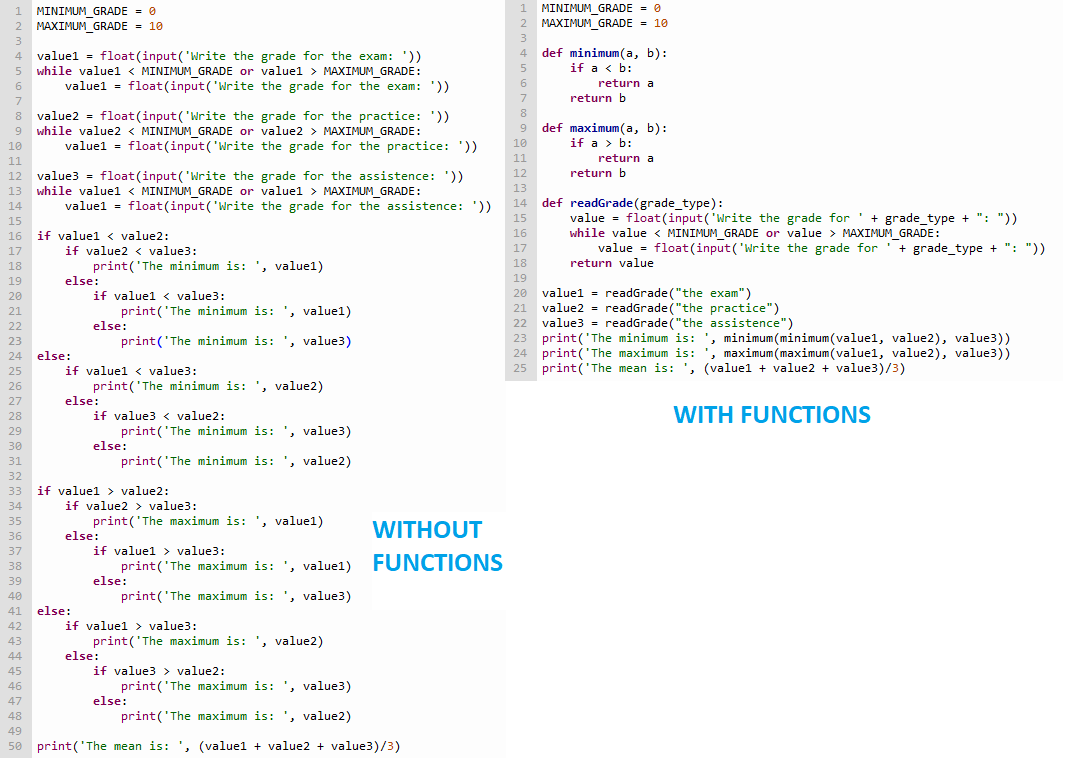
\includegraphics[width=0.90\textwidth]{images/sin-con-funciones-eng.png}
    \caption{Comparison of a program without and with functions}
    \label{fig:sin.con.funciones}
\end{figure}


\section{docstring}
\label{docstring}
\index{docstring}

A {\bf docstring} is a string at the beginning of a function that explains what the function can be used for (``doc'' is short for ``documentation''). Here is an example:

\begin{python}
def minimum(a, b):
    """
    Returns the minimum of the two given numbers.
    """
    if a > b:
        return a
    return b
\end{python}
%
By convention, all docstrings are triple-quoted strings, also known as multiline strings because triple quotes allow the string to be expanded to more than one line.
\index{comillas}
\index{cadena!entre triple comillas}
\index{triple comillas, cadena entre}
\index{cadena!multilínea}
\index{multilínea, cadena}

It's short, but it contains the essential information someone would need to use this feature. It concisely explains what the function does (without going into detail about how it does it). Explain what effect each parameter has on the function's behavior and what type each parameter should be (if it's not obvious).

Writing this type of documentation is an important part of designing the feature. A well-designed function should be simple to explain; If you're having trouble explaining one of your features, perhaps the interface could use some improvement.

Docstrings are accessible with the built-in \pythoninline{help} function.

\begin{Verbatim}[frame=single]
>>> help(minimum)
Help on function minimum in module __main__:

minimum(a, b)
    Returns the minimum of the two given numbers.
\end{Verbatim}






\section{Testing our functions (the pytest module)}


We already know that all the programs we write must be tested to check that the results of our programs match what we expect.
%
When we write programs that we can interact with via the console, we can test our program by entering test input data via the keyboard and checking the resulting output on the screen.
%
However, now when we write functions, we can use the \pythoninline{pytest} module to test their operation.

For example, imagine that we have to write a function \pythoninline{no_vowels} that, given a string \pythoninline{s}, returns the same string \pythoninline{s} but without vowels. For example:

\begin{Verbatim}[frame=single, label = {\em example of execution}]
>>> no_vowels("the water is wet")
  th wtr s wt
\end{Verbatim}

What tests would you run to test your program well? We can try with:

\begin{itemize}[nosep]
    \item the example string \texttt{''the water is wet''}, 
    \item the example starts with a consonant, let's do another test that starts with a vowel
    \item the example ends with a consonant, let's do another test that ends with a vowel
    \item a string that starts and ends with a vowel
    \item the empty string,
     \item a string without spaces,
    \item a string with only one vowel letter,
     \item a string with only one consonant letter,
    \item a string with capital letters
    \item a string that has no vowels
    \item a string that only has vowels
    \item a string with digits
    \item a string with question marks and others
\end{itemize}

We design our test suite by choosing expected input and output values:

\begin{tabular}{|l|l|l|l|}
\hline
test case & input & expected output & comment  \\ \hline\hline
1 & \verb@"the water is wet"@ & \verb@"th wtr s wt"@ & the example string\\
2 & \verb@"is wet the water"@ & \verb@"s wt th wtr"@ & starts with a vowel\\
3 & \verb@"new sentence"@ & \verb@"nw sntnc"@ & ends with a vowel\\
4 & \verb@"another sentence"@ & \verb@"nthr sntnc"@ & ends with a vowel\\
5 & \verb@""@ & \verb@""@ & the empty string\\
6 & \verb@"a"@ & \verb@""@ & only one vowel letter\\
7 & \verb@"m"@ & \verb@"m"@ & only one consonant letter\\
8 & \verb@"astringwithoutspaces"@ &  \verb@"strngwthtspcs"@ & without spaces\\
9 & \verb@"CAPITal letTERS wORk"@ & \verb@"CPTl ltTRS wRk"@ & string with capital letters\\
10 & \verb@"krt yhgf dwpq"@ & \verb@"krt yhgf dwpq"@ & has no vowels\\
11 & \verb@"aeoiuuuoiea"@ & \verb@""@ & only has vowels\\
12 & \verb@"album released in the 80s"@ & \verb@"lbm rlsd n th 80s"@ & with digits\\
13 & \verb@"marks like ? and !"@ & \verb@"mrks lk ? nd !"@ & with question marks and others\\
\hline
\end{tabular}

Imagine that we implement our function in a file called \texttt{no\_vowels.py}

\begin{python}
def no_vowels (s):
    """
    returns the argument s without vowels
    """
    vowels = 'aeiouAEIOU'
    s_noVowels = ''
    for ch in s:
        pos = vowels.find(ch)
        if pos == -1: #ch is not vowel
            s_noVowels = s_noVowels + ch     
    return s_noVowels
\end{python}

We can now run the above tests automatically with pytest, defining:

\begin{python}
import pytest

@pytest.mark.parametrize("test_case, input, expected_output",[
(1, "the water is wet", "th wtr s wt"),             #string example
(2, "astringwithoutspaces", "strngwthtspcs"),       #without spaces
(3, "", ""),                                        #the empty string
(4, "CAPITal letTERS wORk", "CPTl ltTRS wRk"),      #string with capital letters
(5, "krt yhgf dwpq", "krt yhgf dwpq"),              #has no vowels
(6, "aeoiuuuoiea", ""),                             #only has vowels
(7, "album released in the 80s", "lbm rlsd n th 80s"),     #with digits
(8, "marks like ? and !", "mrks lk ? nd !")         #with question marks and others
])

def test_no_vowels(test_case, input, expected_output):
    assert no_vowels(input) == expected_output, "case {0}".format(test_case)
\end{python}

The \pythoninline{pytest.mark.parametrize} allows us to define the test cases (i.e. the expected inputs and outputs) that we want to execute. The first argument to \pythoninline{pytest.mark.parametrize}, ie: \pythoninline{'case_num, input, expected_output'}, reflects the components of the test cases for this function. This is called \emph{test signature} and for this function it matches the first 3 columns of our table above.

\begin{itemize}
    \item \pythoninline{'test_case '}: the identifier/number of the test
    \item \pythoninline{'input'}: the input we want to give to the function
    \item \pythoninline{'expected_output'}: the output we expect to come out
\end{itemize}

The rest of the arguments to \pythoninline{pytest.mark.parametrize} consist of the test cases we have defined.

We then define a test function \pythoninline{test_vowelless} that takes a number of parameters that matches the \emph{test signature}. The only thing the function does is:
\begin{itemize}
    \item call the function we want to test with the inputs \pythoninline{no_vowels(input)}
    \item compare output to expected output \pythoninline{== expected_output}
    \item when the \pythoninline{assert} statement receives a \pythoninline{True} (meaning that the output of the function is what we expected) it does nothing.
    \item when the \pythoninline{assert} instruction receives a \pythoninline{False} (which means that what we expected did NOT come out) then it throws a message indicating that the test case (\pythoninline{case_num}) has failed.
\end{itemize}


The \pythoninline{pytest} module ensures that the test function receives all test cases defined in \pythoninline{pytest.mark.parametrize}. To run the tests we do in the Thonny console:


\begin{Verbatim}[frame=single]
>>> !py.test no_vowels.py
============================= test session starts ==============================
platform darwin -- Python 3.7.9, pytest-6.1.2, py-1.9.0, pluggy-0.13.1
rootdir: /Users/tanjavos/Python/Tema5
collected 8 items

no_vowels.py ........                                                    [100%]
============================== 8 passed in 0.02s ===============================
\end{Verbatim}
    
And we see that the 8 test cases that we have defined have passed. Our program has survived all 8 tests!


\section{CODS, a mnemonic for testing}\label{test-mnemonic}
\index{mnemonic}

To have a little more guidance on what test cases to test with your program, we can use the CODE mnemonic:

\begin{description}
\item[{\color{red} C}]ardinality
\item[{\color{red} O}]rder
\item[{\color{red} D}]omain
\item[{\color{red} E}]ach structure
\end{description}

This mnemonic is inspired by Jeff Langr's book, {\em Pragmatic Unit Testing in Java 8 with JUnit}. The words that make up the mnemonic can help us generate ideas as to which entries to try, just that. It's not guaranteed to come up with ideas, nor does it apply to all possible features, but it's always helpful to be able to start with something that can spark ideas for you.

\subsection{{\color{red} C}ardinality}

In mathematics, the cardinality of a value is the measure of the "number of elements". For example, the string \pythoninline{'abcd'} contains 4 letters, and therefore has cardinality 4. This part of the mnemonic reminds us to try different cardinalities of the inputs. For example,

\begin{itemize}
    \item cardinality 0
    \item cardinality 1
    \item cardinality > 1
\end{itemize}

We recall the function \pythoninline{no_vowels} that given a string \pythoninline{s}, returns the same string \pythoninline{s} but without vowels.

\begin{Verbatim}[frame=single, label = {\em example of execution}]
>>> no_vowels("the water is wet")
  th wtr s wt
\end{Verbatim}

Among the test cases that we saw before, the ones that check different cardinalities for s are:

\begin{tabular}{|l|l|l|l|}
\hline
test case & input & expected output & comment  \\ \hline\hline
1 & \verb@"the water is wet"@ & \verb@"th wtr s wt"@ & cardinality \pythoninline{s} > 1\\
4 & \verb@""@ & \verb@""@ & the empty string, cardinality \pythoninline{s} = 0\\
5 & \verb@"a"@ & \verb@""@ & cardinality \pythoninline{s} = 1, only one vowel letter\\
6 & \verb@"m"@ & \verb@"m"@ & cardinality \pythoninline{s} = 1, only one consonant letter\\
\hline
\end{tabular}


\subsection{{\color{red} O}rder}

For some functions and their solutions, the order of elements is important, for others it is not. In both cases, it is necessary to prove that the method works well.

We recall the function \pythoninline{no_vowels} that given a string \pythoninline{s}, returns the same string \pythoninline{s} but without vowels.

Among the test cases we saw earlier, the ones that check different order of where the vowels are for \pythoninline{s} are:

\begin{tabular}{|l|l|l|l|}
\hline
test case & input & expected output & comment  \\ \hline\hline
1 & \verb@"the water is wet"@ & \verb@"th wtr s wt"@ & starts and ends with consonant\\
2 & \verb@"another sentence"@ & \verb@"nthr sntnc"@ & starts and ends with vowel\\
3 & \verb@"new sentence"@ & \verb@"nw sntnc"@ & starts with a consonant\\
4 & \verb@"is wet the water"@ & \verb@"s wt th wtr"@ & ends with a consonant\\
\hline
\end{tabular}

\subsection{{\color{red} D}omain}

You have to think about whether it is necessary to try different domains of the parameters and their limits.

The specification of the function \pythoninline{no_vowels} clearly says that it has to work when given an argument of type string \pythoninline{s}. So it doesn't really need to work for types int, float, etc. because it is not what the function promises. What we can do is try with strings that contain numbers, to verify that our function works and does not, for example, detect it as vowels or something like that.

Among the test cases we saw earlier, the ones that check for different order of where the vowels are for \pythoninline{s} are:

\begin{tabular}{|l|l|l|l|}
\hline
test case & input & expected output & comment  \\ \hline\hline
11 & \verb@"album released in the 80s"@ & \verb@"lbm rlsd n th 80s"@ & with digits\\
\hline
\end{tabular}


\subsection{{\color{red} E}ach structure}

The structure of the parameters can be very important for the good behavior  of a function. We see that for the function \pythoninline{no_vowels} and the argument \pythoninline{s} of type String, the rest of the test cases that we saw before check different structures of the string \pythoninline{s}:

\begin{tabular}{|l|l|l|l|}
\hline
test case & input & expected output & comment  \\ \hline\hline
7 & \verb@"astringwithoutspaces"@ &  \verb@"strngwthtspcs"@ &  without spaces\\
8 & \verb@"CAPITal letTERS wOR"@ & \verb@"CPTl ltTRS wR"@ &  string with capital letters\\
9 & \verb@"krt yhgf dwpq"@ & \verb@"krt yhgf dwpq"@ & has no vowels\\
10 & \verb@"aeoiuuuoiea"@ & \verb@""@ & only has vowels\\
12 & \verb@"marks like ? and !"@ & \verb@"mrks lk ? nd !"@ & with question marks and others\\
\hline
\end{tabular}





\hypertarget{editor}{%
\section{Debugging}\label{editor}}

\index{depuración}

If you are using a text editor to write your own scripts, you may have problems with spaces and tabs. The best way to avoid these problems is to use spaces exclusively (no tabs). Most text editors that recognize Python do so by default, although there are a few that don't.

\index{espacio en blanco}

Tabs and spaces are usually invisible, which makes it difficult to debug any errors that may occur, so find an editor that handles the indenting for you.

Also don't forget to save your program before running it. Some development environments do this automatically, but others don't. In that case, the program you're seeing in the text editor may not be the one you're actually running.

Debugging can take a long time if you're running the same buggy program over and over again!

Make sure the code you're examining is the same code you're executing. If you're not sure, put something like \texttt{print("hello")} at the top of the program and run it again. If you don't see \texttt{hello} on the screen, you're not running the right program!

\hypertarget{glosario}{%
\section{Glossary}\label{glosario}}

\begin{description}
\item[algorithm]
A general process for solving a category of problems.
\end{description}
\index{algoritmo}

\begin{description}
\item[argument]
A value provided to a function when it is called. That value is assigned to the corresponding parameter in the function.
\end{description}
\index{argumento}

\begin{description}
\item[body]
The sequence of statements within a function definition.
\end{description}
\index{cuerpo}

\begin{description}
\item[composition]
Using an expression or statement as part of a longer one.
\end{description}
\index{composición}

\begin{description}
\item[deterministic]
Pertaining to a program that does the same thing each time it is run, from the same inputs.
\end{description}
\index{determinístico}

\begin{description}
\item[dot notation]
The syntax for calling a function from another module, specifying the module name followed by a dot and the function name.
\end{description}
\index{punto, notación}

\begin{description}
\item[execution flow]
The order in which statements are executed during the operation of a program.
\end{description}
\index{flujo de ejecución}

\begin{description}
\item[fruitful function]
A function that returns a value.
\end{description}
\index{productiva, función}

\begin{description}
\item[function]
A sequence of named statements that perform some useful operation. Functions may or may not take arguments, and may or may not produce a result.
\end{description}
\index{función}

\begin{description}
\item[function call]
A statement that executes a function. It consists of the function name followed by a list of arguments.
\end{description}
\index{función, llamada a}

\begin{description}
\item[function definition]
A statement that creates a new function, specifying its name, parameters, and the statements it executes.
\end{description}
\index{función, definición}

\begin{description}
\item[function object]
A value created by a function definition. The function name is a variable that refers to the function object.
\end{description}
\index{función, definición}

\begin{description}
\item[header]
The first line of a function definition.
\end{description}
\index{cabecera}

\begin{description}
\item[import sentence]
A statement that reads a module file and creates a module object.
\end{description}
\index{import, sentencia} \index{sentencia!import}

\begin{description}
\item[module object]
A value created by an \texttt{import} statement, which provides access to the data and code defined in a module.
\end{description}
\index{módulo}

\begin{description}
\item[parameter]
A name used inside a function to refer to the value passed as an argument.
\end{description}
\index{parámetro}

\begin{description}
\item[pseudo-random]
Pertaining to a sequence of numbers that appear to be random, but are generated by a deterministic program.
\end{description}
\index{pseudoaleatorio}

\begin{description}
\item[return value]
The result of a function. If a function call is used as an expression, the return value is the value of the expression.
\end{description}
\index{valor de retorno}

\begin{description}
\item[void function]
A function that does not return any value.
\end{description}
\index{estéril, función}


\section*{Ejercicios}\label{ejercicios}
\addcontentsline{toc}{section}{Ejercicios}

\begin{ejercicio}
¿Qué mostrará en pantalla el siguiente programa
Python?

\begin{python}
def fred():
   print("Zap")

def jane():
   print("ABC")

jane()
fred()
jane()
\end{python}

a) Zap ABC jane fred jane\\
b) Zap ABC Zap\\
c) ABC Zap jane\\
d) ABC Zap ABC\\
e) Zap Zap Zap
\end{ejercicio}

\begin{ejercicio}Decid que es lo muestra por pantalla el siguiente programa:
\begin{python}
a = 4
def func (x):
    a=a+x
    return a

for cont in range(1,6):
    a=func(cont)
    print(a)
\end{python}

\end{ejercicio}

\begin{ejercicio}
Decid que es lo muestra por pantalla el siguiente programa:
\begin{python}
a = 0
b = 1

def func1 (a):
    b= func2(a+1)+1
	return b

def func2 (a):
	return (b+a)

for cont in range(1,6):
	b= b + func1 (a+1) + 1
    print(b)
\end{python}
\end{ejercicio}

\begin{ejercicio}\label{prod_sin_mult_funciones}
Recuerda el ejercicio \ref{prod_sin_mult}. Donde teniamos que 
implementar un programa que lea dos números enteros y diga si su producto es positivo, negativo, o cero \textbf{sin} llegar a realizar dicho producto. 

Los tests que teníamos que ejecutar ahí para probar que tu programa da las salidas esperadas eran: 
\begin{itemize}
\item primer numero es 0, 
\item segundo numero es 0, 
\item ambos números son 0, 
\item ambos números son positivos, 
\item ambos números son negativos, 
\item primer numero es negativo y segundo es positivo, 
\item primer numero es positivo y segundo es negativo.
\end{itemize}

Re-escribe tu solución para que tenga 2 funciones. Una función estéril \pythoninline{main()} que pide los datos al usuario y le comunica el resltado a traves de la consola. Una función productiva \pythoninline{prod_sin_mult} que implemente la funcionalidad deseada y devuelve el resultado.

Para testear tu solución llama a \pythoninline{main()} y ejecuta los mismos tests de antes en el ejercicio \ref{prod_sin_mult}:\\

\begin{Verbatim}[frame=single, label={\em ejemplos y posibles tests de ejecución}]
>>> main()
  Introduce el primer numero entero: 0
  Introduce el segundo numero entero: -1
  El producto es cero
>>> main() 
  Introduce el primer numero entero: 5
  Introduce el segundo numero entero: 0
  El producto es cero
>>> main() 
  Introduce el primer numero entero: 0
  Introduce el segundo numero entero: 0
  El producto es cero
>>> main() 
  Introduce el primer numero entero: 2
  Introduce el segundo numero entero: 7
  El producto es positivo
>>> main()  
  Introduce el primer numero entero: -4
  Introduce el segundo numero entero: -7
  El producto es positivo
>>> main()  
  Introduce el primer numero entero: -8
  Introduce el segundo numero entero: 3
  El producto es negativo
>>> main()  
  Introduce el primer numero entero: 10
  Introduce el segundo numero entero: -6
  El producto es negativo
\end{Verbatim}
\end{ejercicio}


\begin{ejercicio}\label{dados_rango_play_funciones}
Recuerda el ejercicio \ref{dados_rango_play}. Nos pide un programa para un simple juego de dos dados. El programa tenia que pedir al usuario los dos números de los dados d1 y d2 y decir si el jugador gana (7 o 11), pierde (2, 3 o 12) o si tiene otro chance (4, 5, 6, 8, 9 o 10).

Vamos a re-escribr tu solución para que tenga 3 funciones, una por cada una de las tareas del programa:

\begin{itemize}
    \item Una función estéril \pythoninline{main()} que se encarga de la interacción con el usuario.
    \item Una función productiva \pythoninline{dados_en_rango_correcto} que verifica que los dados están en el rango correcto
    \item Una función productiva \pythoninline{jugar} que solo llamamos cuando los dados están en el rango correcto y que aplica las reglas del juego
\end{itemize}

Para testear tu solución llama a \pythoninline{main()} y ejecuta los mismos tests de antes en el ejercicio \ref{dados_rango_play}:\\


\begin{Verbatim}[frame=single, label={\em example test execution of the program}]
>>> main()
  Valor del dado 1: 2
  Valor del dado 2: 4
  Tienes otra chance!
>>> main()
  Valor del dado 1: 1
  Valor del dado 2: 1
  Perdiste!
>>> main()
  Valor del dado 1: 6
  Valor del dado 2: 5
  Ganaste!
>>> main() 
  Valor del dado 1: 0
  Valor del dado 2: 3
  Error: dado 1 no tiene valor correcto
>>> main() 
  Valor del dado 1: 4
  Valor del dado 2: -8
  Error: dado 2 no tiene valor correcto
>>> main() 
  Valor del dado 1: 50
  Valor del dado 2: -4
  Error: dado 1 no tiene valor correcto
  Error: dado 2 no tiene valor correcto
\end{Verbatim}

\end{ejercicio}



\begin{ejercicio}
Vamos a automatizar la ejecución de los tests de Ejercicio \ref{prod_sin_mult_funciones}

\begin{python}
def prod_sin_mult(n1,n2):
    """
    Recibe dos números enteros y diga si su producto es positivo, negativo, o cero.
    SIN llegar a realizar dicho producto
    """
    #TU SOLUCION aqui

def test_prod_sin_mult():
    assert prod_sin_mult(0, -1) == "El producto es cero"
    assert prod_sin_mult(5, 0) == "El producto es cero"
    assert prod_sin_mult(0, 0) == "El producto es cero"
    assert prod_sin_mult(2, 7) == "El producto es positivo"
    assert prod_sin_mult(-4, -7) == "El producto es positivo"
    assert prod_sin_mult(-8, 3) == "El producto es negativo"
    assert prod_sin_mult(10, -6) == "El producto es negativo"
    
def main():
    n1 = int(input("Introduce primer numero: "))
    n2 = int(input("Introduce segundo numero: "))
    print(prod_sin_mult(n1,n2))
\end{python}
\end{ejercicio}


\begin{ejercicio}  
Vamos a automatizar la ejecución de los tests de Ejercicio \ref{dados_rango_play_funciones}

\begin{small}
\begin{python}
def dados_en_rango_correcto(d1, d2):
    """
    Verifica que dos dados estan dentro del rango correcto
    """
    #COMPLETAR
        
def jugar(d1,d2):
    """
    Aplica las reglas del juego, solo para dados en rango correcto
    """
    #COMPLETAR
  
def main():
    d1 = int(input("Valor del dado 1: "))
    d2 = int(input("Valor del dado 2: "))
    check_dados = dados_en_rango_correcto(d1, d2)
    if (dados_en_rango_correcto(d1, d2) == "Correcto"):
        print(jugar(d1,d2))
    else:
        print(check_dados)
  

def test_dados_en_rango_correcto():
    assert dados_en_rango_correcto(0, 3) == "Error: dado 1 no tiene valor correcto"
    assert dados_en_rango_correcto(5, -4) == "Error: dado 2 no tiene valor correcto"
    assert dados_en_rango_correcto(50, -4) == "Error: dados 1 y 2 no tienen valor correcto"
    assert dados_en_rango_correcto(2, 7) == "Error: dado 2 no tiene valor correcto"
    assert dados_en_rango_correcto(2, 6) == "Correcto"
    assert dados_en_rango_correcto(1, 1) == "Correcto"
    

def test_jugar():
    assert jugar(2, 4) == "Tienes otra chance!"
    assert jugar(1, 1) == "Perdiste!"
    assert jugar(6, 5) == "Ganaste!"    
\end{python}
\end{small}

\end{ejercicio}



\begin{ejercicio}
Escribir una función \pythoninline{my\_pow} que calcule $X^{n}$, tal que $X$ es un número real y $n$ un número entero positivo. Hay que escribir el programa \textit{sin} utilizar la función de librería pythoninline{Math.pow}. Esta función predefinida lo puedes usar en los pytests para chequear la salida de tu función, por ejemplo así:

\begin{small}
\begin{python}
import math
def test_my_pow():
    assert my_pow(2,0) == math.pow(2,0),   "caso Cardinalidad n = 0"
    assert my_pow(0,0) == math.pow(0,0),   "caso Dominio/Cardinalidad X=0 y n=0"
    assert my_pow(0,3) == math.pow(0,3),   "caso Dominio/Cardinalidad X=0, n>1"
    assert my_pow(5,10) == math.pow(5,10), "caso Dominio/Cardinalidad X>1, n>1"
    assert my_pow(-5,6) == math.pow(-5,6), "caso Dominio/Cardinalidad X<0, n>1"
\end{python}
\end{small}

Como vemos en el ejemplo, en Pytest es posible proporcionar un segundo parámetro opcional a la declaración assert. Este parámetro es una cadena de texto que se utiliza para proporcionar un mensaje personalizado en caso de que la afirmación falle.

El mensaje de error personalizado puede ayudar a identificar con mayor precisión la causa del fallo en la prueba. Puedes incluir información adicional relevante o describir la condición esperada que no se cumplió.
\end{ejercicio}



\begin{ejercicio}
Escribir una función (\pythoninline{change_string}) en python que dado un string \pythoninline{cad}, devuelve otro string en que la primera y el ultimo carácter de \pythoninline{cad} se han intercambiado.

También hay que incluir una funcion  pytest \pythoninline{test_change_string}, usando \pythoninline{assert} para probar tu función:

\begin{small}
\begin{python}
import pytest
def test_change_string1():
    assert change_string("") == ""              #Cardinalidad = 0
    assert change_string("z") == "z"            #Cardinalidad = 1
    assert change_string("tanja") == "aanjt"    #Cardinalidad > 1
    assert change_string("abbbba") == "abbbba"  #Orden
    assert change_string("12345") == "52341"    #Dominio
    assert change_string("!@ih&/") == "/@ih&!"  #Estructura
\end{python}
\end{small}

Si lo ejecutamos con pytest sale:

\begin{small}
\begin{python}
>>> %Run change_string.py
>>> !py.test change_string.py
============================= test session starts ==============================
platform darwin -- Python 3.7.9, pytest-6.1.2, py-1.9.0, pluggy-0.13.1
plugins: cov-4.0.0
collected 1 item

change_string.py .                                                       [100%]
============================== 1 passed in 0.01s ===============================
>>> 
\end{python}
\end{small}

Vemos que pytest considera \pythoninline{test_change_string1} con las 6 instruciones \pythoninline{assert} como 1 test. Lo podemos observar porque pone \pythoninline{collected 1 item} and 
\pythoninline{1 passed in 0.01s}.

Recuerda que la otra forma es usar \pythoninline{pytest.mark.parametrize}, lo explicamos otra vez abajo. OJO: si eso te parece todavía muy difícil o confusa, déjalo para más tarde.

\begin{small}
\begin{python}
import pytest
@pytest.mark.parametrize("testcase, entrada, salida_esperada",[
(1, "", ""),               #Cardinalidad = 0
(2, "z", "z"),             #Cardinalidad = 1
(3, "tanja", "aanjt"),     #Cardinalidad > 1
(4, "abbbba", "abbbba"),   #Orden
(4, "12345", "52341"),     #Dominio
(5, "!@ih&/", "/@ih&!")    #Estructura
])

def test_change_string2(testcase, entrada, salida_esperada):
    assert change_string(entrada) == salida_esperada, "caso {0}".format(testcase)
\end{python}
\end{small}


Si lo ejecutamos con pytest sale:

\begin{small}
\begin{python}
>>> %Run change_string.py
>>> !py.test change_string.py
============================= test session starts ==============================
platform darwin -- Python 3.7.9, pytest-6.1.2, py-1.9.0, pluggy-0.13.1
plugins: cov-4.0.0
collected 6 items

change_string.py ......                                                  [100%]

============================== 6 passed in 0.02s ===============================
>>> 
\end{python}
\end{small}

Vemos que pytest considera \pythoninline{test_change_string2} como 6 tests. Lo podemos observar porque pone \pythoninline{collected 6 items} and \pythoninline{6 passed in 0.02s}.

OJO: no olvida importar pytest así:
\pythoninline{import pytest}. Si no lo importas, el interpreter de Python no lo puede encontrar y te dirá: \texttt{NameError: name 'pytest' is not defined}.

\end{ejercicio}



\begin{ejercicio}
Escribir una función (\pythoninline{odd_values_string}) en python que dado un string $s$, devuelve otro string en que los caracteres en las posiciones con index impar se han eliminado. Tu función tiene que pasar tests los siguientes tests:


\begin{small}
\begin{python}
def test_odd_values_string():
    assert odd_values_string("") == ""
    assert odd_values_string("a") == "a"
    assert odd_values_string("aa") == "a"
    assert odd_values_string("abcd") == "ac"
    assert odd_values_string("abcde") == "ace"
    assert odd_values_string("12345") == "135"
    assert odd_values_string("&%$(agt.34") == "&$at3"
    assert odd_values_string("hola espacios  ") == "hl sais "
\end{python}
\end{small}   

Usando \pythoninline{pytest.mark.parametrize} quedaría así:

\begin{small}
\begin{python}
@pytest.mark.parametrize("testcase, entrada, salida_esperada",[
(1, "", ""),                       #Cardinalidad = 0
(2, "a", "a"),                     #Cardinalidad = 1 (0 letras en posición impar)
(3, "aa", "a"),                    #Cardinalidad = 2 (1 letra en posición impar)
(4, "abcd", "ac"),                 #Cardinalidad 2 posiciones impar, 5 letras
(5, "abcde", "ace"),               #Cardinalidad 2 posiciones impar, 5 letras
(6, "12345", "135"),               #Dominio, string con digitos
(7, "&%$(agt.34", "&$at3"),        #Estructura, string con signos
(8, "hola espacios  ", "hl sais ") #Estructura, string con espacios
])

def test_odd_values_string(testcase, entrada, salida_esperada):
    assert odd_values_string(entrada) == salida_esperada,\
           "caso {0}".format(testcase)
\end{python}
\end{small}

\end{ejercicio}

\begin{ejercicio}
Escribir una función \pythoninline{mi_raiz} que calcule la raíz cuadrada de un número $n$, aplicando el método babilónico. Este método consiste en el cálculo de la sucesión $S$:
\begin{center}
$S = \lbrace s_{i} \rbrace ^{\infty}_{i=0}= s_{0} , s_{1} , s_{2} , \dots , s_{\infty}$ donde $: s_{0} = 2 $    y   $ s_{i+1} = \frac {s_{i} + n/s_{i}}{2}$
\end{center}
Cada uno de los términos $s_{i}$ de la serie es una aproximación a $\sqrt{n}$. Evidentemente, el último de los términos calculados será la mejor aproximación. Se calculará un nuevo término $s_{i+1}$ siempre y cuando se cumpla $|s_{i-1} - s_{i} | > 10^{-8}$ .


Puedes usar \pythoninline{math.sqrt} como resultado esperado en tus casos de test. Sin embargo, hay que tener en cuenta que comparar flotantes para la igualdad es un poco complicado debido a problemas de redondeo y precisión.
Podemos comparar que la diferencia entre lo que sale de nuestra función y el \pythoninline{math.sqrt} es menor a por ejemplo $10^{-2}$

\begin{small}
\begin{python}
def test_mi_raiz():
    assert abs(mi_raiz(2) - math.sqrt(2)) < 10**-2, "caso n=2"
    assert abs(mi_raiz(4) - math.sqrt(4)) < 10**-2, "caso n=4"
    assert abs(mi_raiz(7) - math.sqrt(7)) < 10**-2, "caso n=7"
    assert abs(mi_raiz(25) - math.sqrt(25)) < 10**-2, "caso n=25"
    assert abs(mi_raiz(200) - math.sqrt(200)) < 10**-2, "caso n=200"
    assert abs(mi_raiz(1234) - math.sqrt(1234)) < 10**-2, "caso n=1234"
\end{python}
\end{small}
\end{ejercicio}



\begin{ejercicio}
Escribir una función \pythoninline{my\_coseno} que dado un valor real $x > 0$, calcule el coseno de $x$ mediante la siguiente serie:
$$cos(x)=\sum_{i=0}^{\infty}(-1)^{i}\frac{x^{2i}}{(2i)!}= 1 - \frac{x^{2}}{2!} + \frac{x^{4}}{4!} - \dots$$
Se deben calcular términos de la serie mientras el valor absoluto de cada término sea superior a $10^{-7}$.

OJO: Si queremos calcular el coseno de 45 grados usando nuestra función \pythoninline{my\_coseno}, primero tenemos que convertir 45 grados en radianes. Afortunadamente, el módulo matemático de Python tiene una función llamada \pythoninline{math.radians()} que realiza la conversión de ángulos antes.

Aquí puedes usar \pythoninline{math.cos} como resultado esperado en tus casos de test. De nuevo hay que tener en cuenta que comparar flotantes para la igualdad es complicado debido a problemas de redondeo y precisión.
\end{ejercicio}

\begin{ejercicio}
Escribir una función que dado un valor real $x > 0$, calcule el arco-tangente de $x$ mediante la siguiente serie:
$$arctan(x) = \sum_{n=0}^{\infty}(-1)^{i}\frac{x^{2n+1}}{2n+1}= x - \frac{1}{3}x^{3}+\frac{1}{5}x^{5}-\frac{1}{7}x^{7}+\dots$$
Se deben calcular términos de la serie mientras el valor absoluto de cada término sea mayor que $10^{-7}$.

Recuerda usar \pythoninline{math.radians()}. Puedes usar \pythoninline{math.atan} como resultado esperado en tus casos de pytest.
\end{ejercicio}



\begin{ejercicio}
\index{objeto!de función}
\index{función!objeto de}

Un objeto de función es un valor que puedes asignar a una variable o
pasarlo como argumento.  Por ejemplo, \verb"hacer_2veces" es una función
que toma un objeto de función como argumento y lo llama dos veces:

\begin{python}
def hacer_2veces(f):
    f()
    f()
\end{python}

Aquí hay un ejemplo que utiliza \pythoninline{hacer_2veces} para llamar a una función
con nombre \pythoninline{imprimir_spam} dos veces.

\begin{python}
def imprimir_spam():
    print('spam')

hacer_2veces(imprimir_spam)
\end{python}

\begin{enumerate}

\item Escribe este ejemplo en un script y pruébalo.

\item Modifica \pythoninline{hacer_2veces} para que tome dos argumentos, un
objeto de función y un valor, y llame a la función dos veces,
pasando al valor como argumento.

\item Recuerda y copia la definición de
\pythoninline{muestra_dos_veces}, presentada previamente en este tema, a tu script.

\begin{python}[frame=single]
def muestra_dos_veces(bruce):
    print(bruce)
    print(bruce)
\end{python}


\item Usa la versión modificada de \pythoninline{hacer_2veces} para llamar a
\pythoninline{muestra_dos_veces} dos veces, pasando a \pythoninline{'spam'} como argumento.

\item Define una nueva función llamada
\pythoninline{hacer_4veces} que tome un objeto de función y un valor
y llame a la función cuatro veces, pasando al valor
como argumento.  Debería haber solo
dos sentencias en el cuerpo de esta función, no cuatro.

\end{enumerate}

%Solution: \url{http://thinkpython2.com/code/do_four.py}.

\end{ejercicio}

\begin{ejercicio}
\label{anagram}
\index{anagrama}
%
Dos palabras son anagramas si puedes reordenar las letras de una
para escribir la otra.  Escribe una función llamada \pythoninline{es_anagrama}
que tome dos cadenas y devuelva \pythoninline{True} si son anagramas.

En la pagina \url{https://www.ejemplos.co/50-ejemplos-de-anagramas/} puedes encontrar ejemplos de anagramas para escribir tus pytests.


\end{ejercicio}

\begin{ejercicio}
Escribir una función  que, dado un número entero $n$ mayor que cero,
devuelve una lista de los múltiplos de 3 que hay entre 3 y $n$. Escribe otra función que, dado un número entero $n$ mayor que cero, devuelve una lista de los divisores de $n$. Prueba tus funciones con pytest, por ejemplo:

\begin{python}
@pytest.mark.parametrize('testcase, entrada, salida_esperada',[
    (1, 10, [3, 6, 9]),
    (2, 0, []),
    (3, 1, []),
    (4, -5, []),
    (5, 12, [3, 6, 9, 12]),
    (6, 3, [3])
    ])
def test_multiplos_de_3(testcase, entrada, salida_esperada):
    assert multiplos_de_3(entrada)==salida_esperada, 'caso {0}'.format(testcase)

@pytest.mark.parametrize('testcase, entrada, salida_esperada',[
    (1, 10, [1, 2, 5, 10]),
    (2, 18, [1, 2, 3, 6, 9, 18]),
    (3, 1, [1]),
    (4, -5, []),
    (5, 12, [1, 2, 3, 4, 6, 12]),
    (6, 0, [])
    ])
def test_divisores_de(testcase, entrada, salida_esperada):
    assert divisores_de(entrada)==salida_esperada, 'caso {0}'.format(testcase)
\end{python}

Ahora, usa estas funciones para escribir un programa \pythoninline{main} que pide un numero mayor que cero al usuario a través del teclado que devuelve el siguiente:\\

\begin{Verbatim}[frame=single]
>>> %Run 
  Teclea un numero entero mayo a cero: 1
  No hay multiplos de 3
>>> %Run 
  Teclea un numero entero mayo a cero: 2
  No hay multiplos de 3
>>> %Run 
  Teclea un numero entero mayo a cero: 3
  multiplo = 3 divisores del 3 = [1, 3]
>>> %Run 
  Teclea un numero entero mayo a cero: 13
  multiplo = 3 divisores del 3 = [1, 3]
  multiplo = 6 divisores del 6 = [1, 2, 3, 6]
  multiplo = 9 divisores del 9 = [1, 3, 9]
  multiplo = 12 divisores del 12 = [1, 2, 3, 4, 6, 12]
>>> 
\end{Verbatim}


\end{ejercicio}

\begin{ejercicio}
Escribir una función (\pythoninline{letraDNI}) que, dado un número de DNI, devuelva la letra que le corresponde.
%
El algoritmo para calcular la letra de control de un DNI es el siguiente:
\begin{itemize}
\item Calcula el resto de dividir el n\'umero por 23
\item Se obtiene la letra, utilizando el resto como
índice de la siguiente tabla:\\
\end{itemize}

  \begin{tabular}{|c|c|c|c|c|c|c|c|c|c|c|c|c|}
    \hline
    RESTO & 0 & 1 & 2 & 3 & 4 & 5 & 6 & 7 & 8 & 9 & 10 & 11  \\ \hline
    LETRA & T & R & W & A & G & M & Y & F & P & D & X & B  \\ \hline
  \end{tabular}
  
  \begin{tabular}{|c|c|c|c|c|c|c|c|c|c|c|c|}
    \hline
    RESTO & 12 & 13 & 14 & 15 & 16 & 17 & 18 & 19 & 20 & 21 & 22 \\ \hline
    LETRA & N & J & Z & S & Q & V & H & L & C & K & E  \\ \hline
  \end{tabular}\\

Completa la siguiente tabla con la cantidad de filas que ves necesario para diseñar tu conjunto de tests y ejecuta los tests automáticos con pytest.\\

\begin{tabular}{|l|l|l|}
\hline
caso de test número & entrada & salida esperada   \\ \hline\hline
1 & \verb@                      @ & \verb@                       @\\
2 & & \\
3 & & \\
4 & & \\
5 & & \\
6 & & \\
\hline
\end{tabular}


\end{ejercicio}

\begin{ejercicio}
Diseña una función que dado una cadena de texto, devuelve la cantidad de números que aparecen en la cadena. Nota: Con número no queremos decir dígito, sino número propiamente dicho, es decir, secuencia de dígitos. La cadena `un 1, un 201 y 2 unos', por ejemplo, tiene 3 números: el 1, el 201 y el 2.\\

\begin{Verbatim}[frame=single, label={\em ejemplo de ejecuciones}]
>>> nums_en_string("un 1, un 201 y 2 unos")
  3
>>> nums_en_string("sin numeros")
  0
>>> nums_en_string("2345543")
  1
\end{Verbatim}

Escribe pytests para probar tu función de forma automatizado.

\end{ejercicio}

\begin{ejercicio}

Implementa un modulo con un \pythoninline{main} que lea de teclado una cadena que representa un número binario. Si algún carácter de la cadena es distinto de 0 o 1, el programa advertirá al usuario de que la cadena introducida no representa un número binario y pedirá de nuevo la lectura de la cadena. Finalmente, el \pythoninline{main} mostrará el valor entero decimal del número binario introducido.

En el \pythoninline{main} tienes que usar 2 funciones que tienes que definir y testear con pytest en tu modulo:

\begin{itemize}
\item \pythoninline{check_si_es_binario} que dado una cadena de texto devuelve \pythoninline{True} si la cadena esta compuesto por solo 0 y 1, y si no devuelve \pythoninline{False}
\item \pythoninline{convertir} para convertir una cadena en formato binario (i.e. solo 0 y 1) a formato decimal.
\end{itemize}

¿Qué casos de test ejecutarías para probar bien tu main?
¿Y para las 2 funciones? Implementa los tests con pytest.


\end{ejercicio}

\begin{ejercicio}
Implementar una función \pythoninline{fib(n)}
que devuelve una lista con los primeros \pythoninline{n} números de 
Fibonacci. Si \pythoninline{n==0}, la función tiene que devolver la lista 
\pythoninline{[1]}, si \pythoninline{n==1}, la función tiene que devolver la lista\pythoninline{[1,1]}. Cuando \pythoninline{n<1}, entonces hay que empezar con la lista \pythoninline{[1,1]} y añadir el siguiente numero Fibonacci sumando los números anteriores en la lista.

Por ejemplo tecleando:\\

\begin{Verbatim}[frame=single]
>>> print(fib(0))
  [1]
>>> print(fib(1))
  [1, 1]
>>> print(fib(2))
  [1, 1, 2]
>>> print(fib(12))
  [1, 1, 2, 3, 5, 8, 13, 21, 34, 55, 89, 144, 233]
\end{Verbatim}

¡No olvida tus pytests para automatizar los tests!

\end{ejercicio}

\begin{ejercicio}
Escribir una función Python \pythoninline{borrar_negativos} que recibe como argumento una lista y devuelve la misma lista pero sin los elementos negativos.\\

\begin{Verbatim}[frame=single]
>>> borrar_negativos([0,-1,-11,2,33,-100,5])
  [2, 33, 5]
>>> borrar_negativos([-1,-11,-3])
  []
>>> borrar_negativos([4,68,111])
  [4, 68, 111]
\end{Verbatim}

Ejecuta más tests automáticos con pytest. No olvides un tests para la lista vacía y la lista con 1 elemento.

\end{ejercicio}

\begin{ejercicio}
Escribe una función (\pythoninline{posMax}) que dada una lista no vacía devuelva la posición donde se encuentra su valor máximo.
Después, completa la tabla de abajo con la cantidad de filas que ves necesario para diseñar tu conjunto de tests y ejecuta los tests automáticos con pytest. Esta vez no hace falta testear la lista vacía, porque el enunciado dice claramente que tu función solo tiene que funcionar para una lista no vacía.\\

\begin{tabular}{|l|l|l|}
\hline
caso de test número & entrada & salida esperada   \\ \hline\hline
1 & \verb@                      @ & \verb@                       @\\
2 & & \\
3 & & \\
.... & & \\
\hline
\end{tabular}


\end{ejercicio}

\begin{ejercicio}
Escribir una función que dada una lista de palabras y una palabra devuelva el número de veces que aparece dicha palabra en la lista. Después, completa la tabla con la cantidad de filas que ves necesario para diseñar tu conjunto de tests y ejecuta los tests automáticos con pytest.\\

\begin{tabular}{|l|l|l|}
\hline
caso de test número & entrada & salida esperada   \\ \hline\hline
1 & \verb@                      @ & \verb@                       @\\
2 & & \\
3 & & \\
.... & & \\
\hline
\end{tabular}

\end{ejercicio}

\begin{ejercicio}
Diseña una función (\pythoninline{miSplit}) que obtiene una cadena y devuelve una lista con todas sus palabras en minúsculas. La lista devuelta no debe contener palabras repetidas. 
No puedes usar el \pythoninline{split} predefinido de Python.
Por ejemplo, ante la cadena:\\

\begin{Verbatim}[frame=single]
>>> miSplit('Una frase formada con palabras. Otra frase con otras palabras.')
  ['una', 'frase', 'formada', 'con', 'palabras', 'otra', 'otras']
>>> miSplit('Hi! Helloooo HI')
  ['hi', 'helloooo']
\end{Verbatim}

Para diseñar tu conjunto de tests que tienes que ejecutar de forma automáticos con pytest piensa en casos:

\begin{itemize}[nosep]
    \item que la cadena es vacía
    \item que la cadena tiene signos de puntuación, como  \verb|,;.:-¿?+*()!¡|
    \item que la cadena termine con un punto
    \item que la cadena no termine con un punto
    \item que la cadena tiene números
    \item que la cadena tiene palabras repetidos, pero unos tiene mayúsculas y otras no (por ejemplo: \pythoninline{'HOla hola hoLa'}
    \item que la cadena tiene más de 1 espacio entre palabras
    \item etc.
\end{itemize}


\end{ejercicio}

\begin{ejercicio}
Escribir una función que dada una lista de números devuelva otra lista sin los números impares. 
Después, completa la tabla con la cantidad de filas que ves necesario para diseñar tu conjunto de tests y ejecuta los tests automáticos con pytest.\\

\begin{tabular}{|l|l|l|}
\hline
caso de test número & entrada & salida esperada   \\ \hline\hline
1 & \verb@                      @ & \verb@                       @\\
2 & & \\
3 & & \\
.... & & \\
\hline
\end{tabular}

\end{ejercicio}

\begin{ejercicio}
Escribir una función que dada una lista de números devuelva otra lista sin elementos repetidos. Después, completa la tabla con la cantidad de filas que ves necesario para diseñar tu conjunto de tests y ejecuta los tests automáticos con pytest.\\

\begin{tabular}{|l|l|l|}
\hline
caso de test número & entrada & salida esperada   \\ \hline\hline
1 & \verb@                      @ & \verb@                       @\\
2 & & \\
3 & & \\
.... & & \\
\hline
\end{tabular}


\end{ejercicio}

\begin{ejercicio}
Escribir un modulo con tres funciones y sus pytest sobre matrices: \pythoninline{sum\_of\_diagonal}, \pythoninline{create\_matriz} y \pythoninline{multiplicar}.

1) La primera función es (\pythoninline{sum\_of\_diagonal}) que dado una matriz $m$ de integers calcula la suma de los integers que están en el diagonal. Tu función tiene que comprobar que la matriz es cuadrada y efectivamente tiene un diagonal para sumar. Por ejemplo:

$
{\texttt{tt sum\_of\_diagonal}}(
\begin{bmatrix}
    1 & 2 & 3 & 4 \\
    2 & 4 & 6 & 1 \\
    0 & 5 & 8 & 2 \\
    2 & 9 & 6 & 3 \\
\end{bmatrix})
 = 16
$, $\;\;$
$
{\texttt{sum\_of\_diagonal}}(
\begin{bmatrix}
    1 & 5   \\
    3 & 4  \\
\end{bmatrix})
 = 5
$

Tu función tiene que pasar los siguientes tests:

\begin{small}
\begin{python}
@pytest.mark.parametrize("testcase, input, output",[
(1, [[1,2,3],[4,5,6],[7,8,9]], 15),
(2, [[1,0,1],[1,1,0],[1,1,1]], 3),
(3, [[2,0],[0,2]], 4),
(4, [[2,0],[0,2,3]], "matriz no es cuadrada"),
(5, [], 0)]

def test_sum_of_diagonal(testcase, input, output):
    assert sum_of_diagonal(input) == output,\
           "caso {0}".format(testcase)
\end{python}
\end{small}

2) Después, escribimos una función (\pythoninline{create\_matriz}) que dado dos números $n$ y $m$ devuelve una lista que representa una matriz con $n$ filas y $m$ columnas con todos el valor 0.

$
{\texttt{create\_matrix}}(3,4) = 
\begin{bmatrix}
    0 & 0 & 0 & 0 \\
    0 & 0 & 0 & 0 \\
    0 & 0 & 0 & 0 \\
\end{bmatrix})
$

Diseñar un conjunto de casos de test y automatizarlos con el pytest.

3) La tercera función es para (\pythoninline{multiplicar}), dado dos matrices $m_1$ y $m_2$ devuelve $m_1 \times m_2$. Recuerda\footnote{\url{https://es.wikipedia.org/wiki/Multiplicación_de_matrices}}
que solo podemos multiplicar 2 matrices si el número de columnas de la matriz $m_1$ es igual al número de filas de la matriz $m_2$.\\

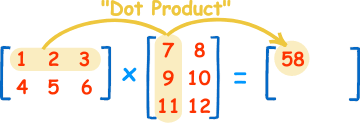
\includegraphics[width=0.5\textwidth]{book/Spanish/05_Funciones/images/mult-matrix.png}

Tu función tiene que pasar los siguientes tests:

\begin{small}
\begin{python}
@pytest.mark.parametrize("testcase, input1, input2, output",[
(1, [[12,7,3], 
     [4, 5,6], 
     [7, 8,9]],
    [[5,8,1,2],
     [6,7,3,0],
     [4,5,9,1]],
    [[114, 160,  60, 27], 
     [ 74,  97,  73, 14], 
     [119, 157, 112, 23]]
),
(2, [[12,7,3, 0], 
     [ 4,5,6,12], 
     [ 6,7,8, 9]
    ],
    [[8,5,8,1,2],
     [6,9,7,3,0],
     [4,5,9,1,0],
     [4,5,9,1,0]
    ],
    [[150, 138, 172, 36, 24], 
     [134, 155, 229, 37, 8], 
     [158, 178, 250, 44, 12]
    ]
),
(3, [], [], []
),
(4,[[]],[[]], "no se pueden multiplicar"
),
(5, [[]],[[[]]], "no se pueden multiplicar"
),
(6, [[[]]],[[]], [[]]
)
])

def test_multiplicar(testcase, input1, input2, output):
    assert multiplicar(input1, input2) == output, 
           "caso {0}".format(testcase)
\end{python}
\end{small}


\end{ejercicio}


\section*{Más ejercicios: Practicar, practicar, practicar!}
\addcontentsline{toc}{section}{Más ejercicios: Practicar, practicar, practicar!}


\begin{ejercicio}Escribe una función con pytests  que reciba una lista de enteros \verb#v# y
   un entero \verb#x# y devuelva el n\'umero de apariciones de \verb#x# en \verb#v#.
\end{ejercicio}


\begin{ejercicio}Escribe una función con pytests  que reciba una lista de enteros
  \verb#v# y devuelva el n\'umero m\'aximo almacenado en el vector.
\end{ejercicio}

\begin{ejercicio}Escribe una función con pytests  que reciba una lista de enteros
  \verb#v# y devuelva el segundo mayor n\'umero almacenado en
  el vector (supondremos que el tama\~no de la lista es por lo menos 2).
\end{ejercicio}
\begin{ejercicio}Escribe una función con pytests  que reciba una lista de enteros
  \verb#v# y devuelva el n\'umero de elementos impares en
  posiciones pares.
\end{ejercicio}
\begin{ejercicio}Escribe una función con pytests  que reciba una lista de enteros
  \verb#v# y dos enteros \verb#x# y \verb#n#, y devuelva el n\'umero
  de elementos de \verb#v# menores que \verb#x# que se encuentren en
  posiciones anteriores a \verb#n#.
\end{ejercicio}
\begin{ejercicio}Escribe una función con pytests  que reciba una lista de enteros
  \verb#v# y devuelva si est\'a ordenado de forma
  ascendente.
\end{ejercicio}

\begin{ejercicio}Escribe una función con pytests  que reciba una lista de enteros
  \verb#v# y devuelva la posici\'on (si existe, de lo contrario
  devuelve -1) de la primera subsecuencia de la lista con tres
  valores iguales consecutivos.
\end{ejercicio}
\begin{ejercicio}Adapta tu anterior función y los pytests  para que también reciba un numero $n$ que indica la longitud deseada de la subsecuencia. (Es decir si $n=3$ sale lo mismo que la función anterior).
\end{ejercicio}

\begin{ejercicio}Escribe una función con pytests  que reciba una lista de enteros
  \verb#v# y un n\'umero entero no negativo \verb#x# y devuelva si
  la suma de los elementos de la lista es mayor que \verb#x#.
\end{ejercicio}
\begin{ejercicio}Escribe una función con pytests  que reciba una lista de \emph
  {enteros no negativos} \verb#v# y un n\'umero entero no negativo
  \verb#x# y devuelva si la suma de los elementos de la lista es
  mayor que \verb#x#; \textbf{analizar el menor n\'umero de posiciones de} \verb#v#.
\end{ejercicio}
\begin{ejercicio}Escribe una función con pytests  que reciba una lista de enteros
  \verb#v# y dos enteros \verb#x# y \verb#n#, y devuelva la primera
  posici\'on de la subsecuencia de \verb#n# valores consecutivos
  mayores que \verb#x#, o -1 cuando subsecuencia que no est\'a
  presente.
\end{ejercicio}
\begin{ejercicio}Escribe una función con pytests  que reciba una lista de enteros
  \verb#v# y devuelva el n\'umero de ceros consecutivos que est\'an en
  el extremo de la lista, usando el menor n\'umero posible de
  operaciones.
\end{ejercicio}
\begin{ejercicio}Escribe una función con pytests  que reciba una lista de enteros
  \verb#v# y devuelva la posici\'on del \'ultimo elemento impar en
  \verb#v# (o -1 si no hay elementos impares).
\end{ejercicio}
\begin{ejercicio}Escribe una función con pytests  que reciba una lista de enteros
  \verb#v# y devuelva la suma de todos los elementos que aparecen
  despu\'es del primer elemento impar.
\end{ejercicio}

\begin{ejercicio}Escribe una función con pytests  que reciba una lista de enteros
   \verb#v# y dos enteros \verb#i# y \verb#f# (0 $\le$ \verb#i# $\le$
   \verb#f# $\le$ \verb#len(v)-1#), y devuelve la lista en que están multiplicados por dos
   los elementos de \verb#v# entre esas dos posiciones \verb#i# y
   \verb#f#.
\end{ejercicio}
\begin{ejercicio}Escribe una función con pytests  que reciba una lista de enteros
   \verb#v# y dos enteros \verb#i# y \verb#f# (0 $\le$ \verb#i# $\le$
   \verb#f# $\le$ \verb#len(v)-1#), y devuelve la lista en que están invertido los elementos
   de la lista entre esas dos posiciones (es decir, el elemento
   \verb#v[i]# se intercambiar\'a con \verb#v[f]#, \verb#v[i+1]# con
   \verb#v[f-1]#, etc.)
\end{ejercicio}
\begin{ejercicio}Escribe una función con pytests  que reciba una lista de enteros
  \verb#v# y dos enteros \verb#i# y \verb#f# (0 $\le$ \verb# i# $\le$
  \verb# f# $\le$ \verb#len(v)-1#), y devuelve la lista en que esta desplazado una
  posici\'on a la derecha todos los elementos de la lista entre esas
  dos posiciones (ambas incluidos); el movimiento debe ser circular
  (es decir, el elemento en la posici\'on \verb#f# ser\'a finalmente en
  la posici\'on \verb#i#).
\end{ejercicio}
\begin{ejercicio}Escribe una función con pytests  que reciba una lista de enteros
  \verb#v# y dos enteros \verb#i# y \verb#f#(0 $\le$ \verb#i#$\le$
  \verb#f# $\le$ \verb#len(v)-1#), y devuelve la lista en que esta desplazado una
  posici\'on a la izquierda, todos los elementos de la lista entre
  esas dos posiciones (ambas incluidos); el movimiento debe ser
  circular (es decir, el elemento en la posici\'on \verb#i# quedar\'a
  finalmente en la posici\'on \verb#f#).

\end{ejercicio}
\begin{ejercicio}Escribe una función con pytests  que reciba dos listas de
  n\'umeros enteros de la misma longitud y devuelva el producto
  escalar.
\end{ejercicio}
\begin{ejercicio}Implementar un una función con pytests  que reciba dos listas de
  \texttt{float} y devuelva si el primero es un prefijo del
  segundo, es decir, todos los elementos del primero est\'an en el
  mismo orden en el comienzo de el segundo.
\end{ejercicio}
\begin{ejercicio}Implementar un una función con pytests  que reciba una lista de enteros \verb#a# con \verb#len(a)# $>0$,
  donde todos sus elementos est\'an entre 0 y 9 (incluidos). La función devuelve los primeros elementos de la
lista donde no hay elementos consecutivos repetidos, por ejemplo:

\begin{itemize}
\item Cuando \verb#a# es \verb#[8,8,4,3]#, El resultado es \verb#8#
\item Cuando \verb#a# es \verb#[4,0,5,9,9]#, El resultado es  \verb#4059#
\item Cuando \verb#a# es \verb#[0,9,4,5,9]# El resultado es  \verb#09459#
\item Cuando \verb#a# es \verb#[1,7,1,0,0,8,7[# El resultado es \verb#1710#
\end{itemize}
\end{ejercicio}

\begin{ejercicio}Implementar un una función con pytests  que reciba una lista \verb#a# de n\'umeros enteros, y devuelva la suma de los elementos que son sim\'etricos e iguales
en la lista \verb#a#. En el caso de que haya un n\'umero impar de
elementos, el elemento central es considerado sim\'etrico e igual
a s\'i mismo. Por ejemplo:


\begin{itemize}
\item Cuando \verb#a# es \verb#[1,2,3,2,1]#  devuelve \verb#9#
\item Cuando \verb#a# es \verb#[1,2,3,2,5]# devuelve \verb#7#
\item Cuando \verb#a# es \verb#[1,2,3,5,1]# devuelve \verb#5#
\item Cuando \verb#a# es \verb#[1,2,3,2]# devuelve \verb#0#
\item Cuando \verb#a# es \verb#[1,2,3,1]# devuelve \verb#2#
\end{itemize}
\end{ejercicio}

\begin{ejercicio}Escribe un una función con pytests con el siguiente encabezado:

\begin{verbatim}
def detect(s1, s2):
\end{verbatim}

cuyos par\'ametros son dos listas de caracteres.
La función debe devolver \verb#true# cuando la secuencia de caracteres
almacenada en \verb#s1# est\'a en \verb#s2#, aunque no est\'e presente
como un bloque \'unico, es decir, puede estar fragmentado, pero en
el mismo orden. Por ejemplo,``Castor'' est\'a presente en `` Ayer en
\textbf{Cas}ablanca hab\'ia \textbf{tor}menta'', pero no en `` Ayer fue un d\'ia
tormentoso en Casablanca''.

\end{ejercicio}

\begin{ejercicio}Implementar una función con pytests  que reciba una matriz de
  \texttt{float} y devuelva una lista que contiene la suma de cada
  columna de la matriz.
\end{ejercicio}
\begin{ejercicio}Implementar una función con pytests  que reciba una matriz de
  \texttt{float} y devuelva una lista que contenga los elementos
  m\'aximos para cada fila de la matriz.
\end{ejercicio}
\begin{ejercicio}Implementar una función con pytests  que reciba una matriz de
  \verb#int# y devuelva si cualquier elemento en la posici\'on
  \verb#[i][j]# es igual a la suma de todos los elementos de la
  submatriz de \verb#[0][0]# a \verb#[i-1]# [j-1].

\end{ejercicio}
\begin{ejercicio}Implementar una función con pytests  que reciba una matriz de
  \verb#double# y un par de enteros (posici\'on), y devuelva la suma
  de la submatriz 3$\times$3 centrada en la posici\'on dada. Si la
  posici\'on est\'a en cualquier frontera de la matriz, la submatriz debe
  limitarse a tomar s\'olo posiciones que realmente existe en la
  matriz.
\end{ejercicio}

\begin{ejercicio}\label {lastmatrix} Implementar una función con pytests  que reciba
  una matriz de \verb#double# y devuelva la columna con la suma
  m\'inima de su elementos.
\end{ejercicio}

\begin{ejercicio}Implementar una función con pytests que, dado una lista de \verb#char#,
  \verb#palabra# y una matriz tambi\'en de \verb#char#, donde el
  tama\~no de todas las filas es igual a la longitud de
  \verb#palabra#, busque iterativamente si \verb#palabra# es igual,
  carácter a carácter, a cualquier fila de la matriz. El m\'etodo debe
  devolver el \'indice de la primera fila en la que existe
  coincidencia. De lo contrario, debe devolver -1. 

\end{ejercicio}

\section*{Ejercicios de tipo test}\label{ejercicios_tipo_test}
\addcontentsline{toc}{section}{Ejercicios de tipo test}

\begin{ejercicio}
Considera el siguiente programa Python:

\begin{python}
def funcion(x):
  # cuerpo
print(funcion(3.5) + 6)
\end{python}

¿Cuál podía ser su cuerpo?:

\begin{choices}
    \choice \pythoninline{return "x"}
    \choice \pythoninline{print(x)}
    \choice \pythoninline{return x} %correct
    \choice \pythoninline{print("x")}
\end{choices}
\end{ejercicio}


\begin{ejercicio}
¿Qué imprime por pantalla el siguiente programa?

\begin{python}
num = 5
def func():
     print(num)
     num = 6
func()
print(num)
\end{python}


\begin{choices}
    \choice 6 \\ 5
    \choice 5 \\ 6
    \choice sale un error %\CorrectChoice
    \choice 6 \\ 6
\end{choices}

\end{ejercicio}

\begin{ejercicio}  ¿Qué es lo que NO forma parte de la cabecera de una función?:

\begin{choices}
    \choice nombre de la función
    \choice valor de retorno   %CORRECT
    \choice lista de parámetros
    \choice palabra clave \texttt{def}
\end{choices}
\end{ejercicio}


\begin{ejercicio} 
Imagine las siguientes instrucciones en Python:

\begin{python}
def hello(x):
    global var
    var+=1
    print(var, x)
var=12
x = var
hello("x")
\end{python}

¿Cuál es el resultado?

\begin{choices}
    \choice \pythoninline{13 x} %CORRECT
    \choice \pythoninline{Error}
    \choice \pythoninline{13 12}
    \choice \pythoninline{13}
\end{choices}

\end{ejercicio}


\begin{ejercicio} Considera el siguiente código Python en el fichero 
\pythoninline{code.py}:

\begin{python}
import pytest
def do_something(s):
  global suma
  suma = 0
  res = "0"
  for i in range(1, len(s)-1):
    if i % 3 == 0:
      suma = suma + int(s[i])
      res = res + s[i]
      print(res)
  return str(suma) + res

@pytest.mark.parametrize("tc_id, entrada, salida_esperada",[
(1, "12345", "404"),
(2, "012345012345", "60303"),
(3, "-1256", "505"),
(4, "", "0")])

def test_values_string(tc_id, entrada, salida_esperada):
    assert do_something(entrada) == salida_esperada
\end{python}

¿Cuál es el resultado cuando llamamos a \pythoninline{\!py.test code.py}?

\begin{choices}
    \choice  1 failed, 3 passed in 0.14s   %CORRECT
    \choice  2 failed, 2 passed in 0.14s
    \choice  3 failed, 1 passed in 0.14s
    \choice  4 passed in 0.14s
\end{choices}

\end{ejercicio}

\begin{ejercicio} Considera el siguiente código Python en el fichero 
\pythoninline{values_string.py}:

\begin{python}
import pytest

def values_string(s):
  result = "" 
  for i in range(len(s)):
    if i % 2 == 0:
      result = result + s[i]
  return result

@pytest.mark.parametrize("tc, entrada, salida",[
(1, "12345", "135"),
(2, "01234567", "1357"),
(3, "-112241", "-11"),
(4, "", "")])

def test_values_string(tc, entrada, salida):
    assert values_string(entrada) == salida, "caso {0}".format(tc)
\end{python}

¿Cuál es el resultado cuando llamamos a \pythoninline{\!py.test values_string.py}?

\begin{choices}
    \choice  2 failed, 2 passed in 0.14s %CORRECT
    \choice  1 failed, 3 passed in 0.14s
    \choice  3 failed, 1 passed in 0.14s
    \choice  4 passed in 0.14s
\end{choices}


\end{ejercicio}


\begin{ejercicio}  Considera el siguiente programa Python:

\begin{python}
def func(y, x = 1):
    y = 2
    x = x + y
    y += 1
    print(x)
\end{python}

¿Qué imprime cuando llamamos a \verb|func(4)|?

\begin{choices}
    \choice 3   %CORRECT
    \choice 6
    \choice 7
    \choice 4
\end{choices}

\end{ejercicio}

\begin{ejercicio} Considera los siguientes tests y test driver:

\begin{small}
\begin{python}
@pytest.mark.parametrize("n, a, b, c, o",[
(1, 3, [3,5], 2.4, "hola"),
(2, 5, "a", 3.0, "onetwoone")
])
def test_funcionX(n, a, b, c, o):
    assert funcionX(a, b, c) == o,  "test {0}".format(n)
\end{python}
\end{small} 

Considerar también las siguientes funciones:

\begin{small}
\begin{python}
def funcion1(a):
    print("hola")

def funcion2 (a, b):
    return "hi" + a + b

def funcion3(a, b, c):
    return str(a) + "onetwoone"

def funcion4 (a, b, c, d):
    return "hola"
\end{python}
\end{small} 

El driver \pythoninline{test_funcionX} solo puede ser para testear la \pythoninline{funcionX} con X igual a:

\begin{choices}
    \choice 3   %CORRECT
    \choice 1
    \choice 2
    \choice 4
\end{choices}
\end{ejercicio}



\begin{ejercicio} Mira el siguiente esquema con las cajas numeradas.

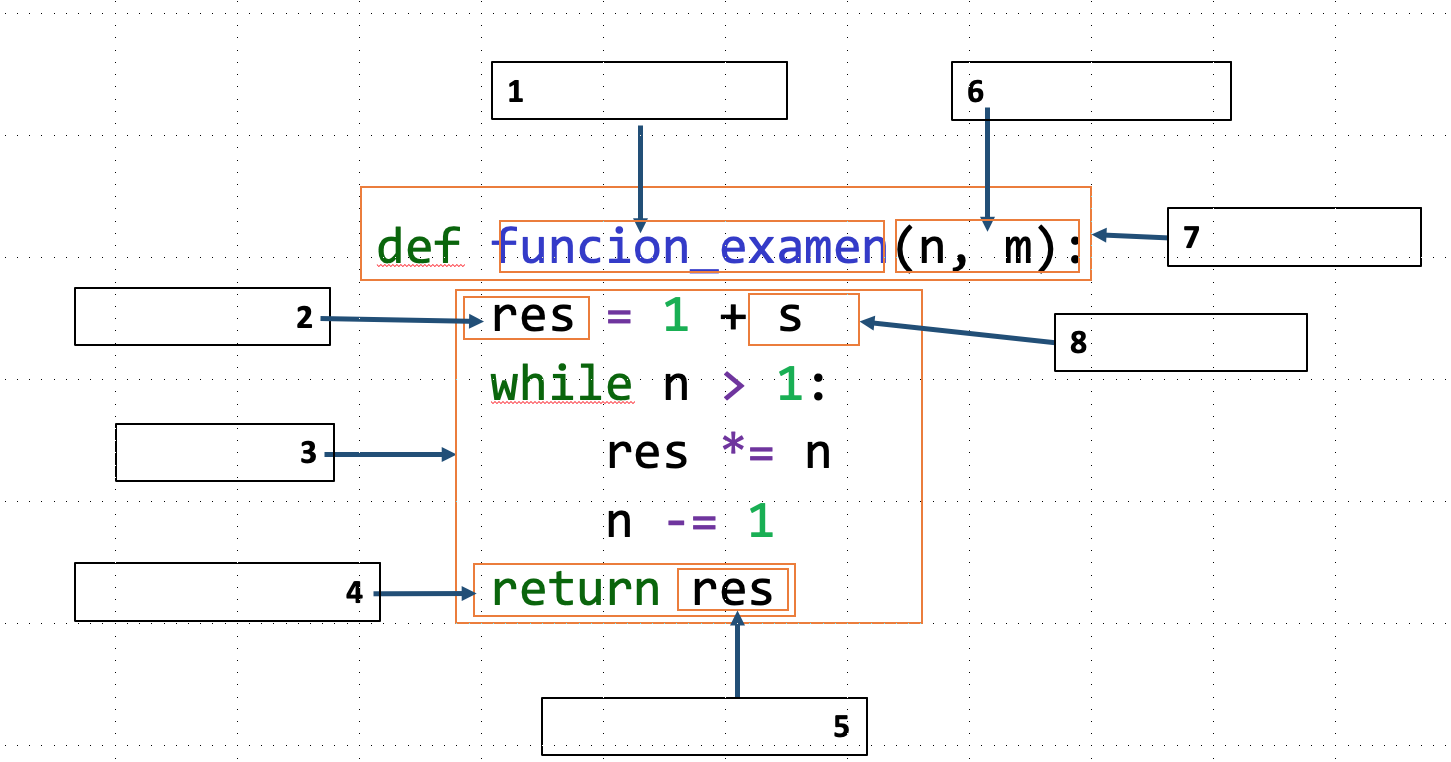
\includegraphics[width=0.5\textwidth]{book/Spanish/05_Funciones/images/funcion.png}

¿Cuál de los siguientes es correcto?

\begin{choices}
    \choice caja 1 contiene el nombre de la función, res es una variable local, caja 3 contiene el cuerpo, caja 6 tiene los parametros   %CORRECT
    \choice caja 1 representa la cabecera, n es una variable global, cajita 3 contiene el cuerpo, s es una variable global
    \choice cala 4 contiene la instrucción de retorno, caja 5 contiene el valor devuelto, variables n y m siempre tiene que ser global  
    \choice res es una variable global, caja 4 contiene la instrucción de retorno, caja 5 contiene el valor devuelto, s es una variable local

\end{choices}
\end{ejercicio}




%\printbibliography
\end{document}


